

\documentclass[landscape,a0b,final,a4resizeable]{include/a0poster}

\usepackage{float}
\usepackage{subfigure}
\usepackage{multicol}
\usepackage{color}
\usepackage{geometry}
\geometry{paperwidth=72in,paperheight=36in,margin=4cm}
\usepackage{morefloats}
\usepackage{setspace}
\usepackage[pdftex]{graphicx}
\usepackage{rotating}
\usepackage{amsmath, amsthm, amssymb, bm}
\usepackage{array}
\usepackage{booktabs}
\usepackage{multirow}
\usepackage{hyperref}

\newcommand{\bP}{\mathbb{P}}
\newcommand{\bQ}{\mathbb{Q}}
\newcommand{\Reg}{\varepsilon}
\newcommand{\diff}{\,\mathrm{d}}
\usepackage{include/picins}
\usepackage{tikz}
\usetikzlibrary{shapes.geometric,arrows,chains,matrix,positioning,scopes,calc}
\tikzstyle{mybox} = [draw=white, rectangle]
\definecolor{darkblue}{rgb}{0,0.08,0.45}
\definecolor{blue}{rgb}{0,0,1}



\usepackage{mathtools}
\usepackage{tcolorbox}

\usepackage{dsfont}




\newcommand{\myfig}[3][0]{
\begin{center}
  \vspace{1.5cm}
  \includegraphics[width=#3\hsize,angle=#1]{#2}
  \nobreak\medskip
\end{center}}


\setcounter{figure}{1}
\newcommand{\mycaption}[1]{
  \vspace{0.5cm}
  \begin{quote}
    {{\sc Figure} \arabic{figure}: #1}
  \end{quote}
  \vspace{1cm}
  \stepcounter{figure}
}


\definecolor{camlightblue}{rgb}{0.601 , 0.8, 1}
\definecolor{camdarkblue}{rgb}{0, 0.203, 0.402}
\definecolor{camred}{rgb}{1, 0.203, 0}
\definecolor{camyellow}{rgb}{1, 0.8, 0}
\definecolor{lightblue}{rgb}{0, 0, 0.80}
\definecolor{white}{rgb}{1, 1, 1}
\definecolor{whiteblue}{rgb}{0.80, 0.80, 1}


\setlength{\columnsep}{0.03\textwidth}
\setlength{\columnseprule}{0.0018\textwidth}
\setlength{\parindent}{0.0cm}


\tikzstyle{mysection} = [rectangle, 
			draw=none, 
			shade, 
			outer color=camlightblue!30,
			inner color=camlightblue!30,
			text width=0.965\columnwidth,
			rounded corners=20pt,
			minimum height=0.08\columnwidth]

\newcommand{\mysection}[1]
{
\begin{center}
  \begin{tikzpicture}
    \node[mysection] {\sffamily\bfseries\huge#1};
  \end{tikzpicture}
\end{center}
}


\renewcommand{\familydefault}{cmss}
\sffamily


\newcommand{\background}[3]{
}





\newenvironment{pcolumn}[1]{
  \begin{minipage}{#1\textwidth}
  \begin{center}
}{
  \end{center}
  \end{minipage}
}




\definecolor{lcolor}{rgb}{0, 0, 0.80}
\definecolor{gcolor1}{rgb}{1, 1, 1}
\definecolor{gcolor2}{rgb}{.80, .80, 1}


 

\newcommand{\pbox}[4]{
\mbox{
\begin{minipage}[t][#2][t]{#1}
#4
\end{minipage}
}%
}


\newenvironment{poster}{
  \begin{center}
  \begin{minipage}[c]{\textwidth}
}{
  \end{minipage}
  \end{center}
}

\def\newarrow{\mbox{\begin{tikzpicture}
             \useasboundingbox{(-3pt,-4.5pt) rectangle (19pt,1pt)};
             \draw[->] (0,-0.07)--(17pt,-0.07);\end{tikzpicture}}}





\makeatletter%
\newlength{\nonHumbleHeight}
\def\@humbleformat#1{{\settoheight{\nonHumbleHeight}{#1}\resizebox{!}{0.94\nonHumbleHeight}{#1}}}%
\def\humble#1{\@humbleformat{#1}}%
\makeatother%
\newcommand{\orho}{\overline{\rho}}
\newcommand{\gp}{{\humble GP}}
\newcommand{\gpt}{{\sc gp}}
\newcommand{\MLP}{{\humble MLP}}
\newcommand{\hx}{\hat{x}}
\newcommand{\hP}{\widehat{\mathbb{P}}}


\newcommand\transpose{{\textrm{\tiny{\sf{T}}}}}
\newcommand{\note}[1]{}
\newcommand{\hlinespace}{~\vspace*{-0.15cm}~\\\hline\\\vspace*{0.15cm}}
\newcommand{\embeddingletter}{g}
\newcommand{\bo}{{\sc bo}}
\newcommand{\agp}{Arc \gp}






\newcommand{\D}{\mathcal{D}}
\newcommand{\X}{\mathbf{X}}
\newcommand{\y}{y}
\newcommand{\data} {\X, \y}
\newcommand{\x}{\mathbf{x}}
\newcommand{\f}{\mathit{f}}


\newcommand{\candidates} {\mathbf{X}_c}
\newcommand{\starts}{\mathbf{X}_s}
\newcommand{\levels}{\mathbf{y}_d}
\newcommand{\lengthScales}{\mathbf{L}_l}
\DeclarePairedDelimiterX{\inp}[2]{\langle}{\rangle}{#1, #2}
\newcommand{\fx}{ f(\mathbf{x}) }
\newcommand{\U}{\mathcal{U}}
\newcommand{\E}{\mathbf{E}}


\definecolor{k4}{HTML}{21304D}
\definecolor{DirtyGreen}{HTML}{CDDA70}
\definecolor{WinterSkin}{HTML}{EFE4CA}
\definecolor{Smak}{HTML}{790800}
\begin{document}
\pagecolor{DirtyGreen!0}

\begin{poster}

\vspace{-0.8\baselineskip}




\begin{center}
\begin{tikzpicture}[x=0.4\textwidth]
    \node at (+1, 0) {};    
    \node at (-1, 0) {};
    \def \badgeheight {0.06\textwidth}
    \node[inner sep=0,text width=0.5\textwidth,text centered,font=\Huge] (Title) at (0,0) 
    {
        {\sffamily\fontsize{80pt}{80pt} \textbf{Sinkhorn Distributionally Robust Optimization}}\\
        {\sffamily\fontsize{60pt}{60pt} Jie Wang${}^{\mbox{$\dagger$}}$, Rui Gao$^{\mbox{$\ddagger$}}$, Yao Xie${}^{\mbox{$\dagger$}}$}\\
        {\sffamily\LARGE $\dagger$~H. Milton Stewart School of Industrial and Systems Engineering, Georgia Institute of Technology}
    \\
    {\sffamily\LARGE $\ddagger$~Department of Information, Risk, and Operations Management, McCombs School of Business, University of Texas at Austin}
    };
    \node [mybox] (Cambridge Badge) at (-0.9, 0) {
        
\includegraphics[height=0.03\textwidth]{figures/Fig_logo_1}
    };
    \node [mybox] (CBL Badge) at (+0.9, 0) {
        
\includegraphics[height=0.07\textwidth]{figures/QR_hist}
    };
\end{tikzpicture}
\end{center}



\vspace*{-1cm}

\Large




\begin{multicols}{4}



\mysection{Contributions}

\vspace{0.1in}
{\LARGE
\begin{itemize}
	\item Distributionally robust optimization with entropic regularized Wasserstein distance (Sinkhorn distance).\vspace{0.1in} 
	\item Ambiguity set contains only absolutely continuous distributions.\vspace{0.1in} 
	\item Computationally efficient first-order optimization algorithm.
\end{itemize}
}
\vspace{0.5in}

\mysection{Decision-Making Under Uncertainty}
\vspace{0.1in} 


\begin{itemize}
\item
{
\LARGE
Objective: Find decision $\theta$ to minimize the risk
\[
\mathcal{R}(\theta;\mathbb{P}) = \mathbb{E}_{\mathbb{P}}\big[f_{\theta}(z)\big].
\]
}
\item
{
\LARGE
Available Information:
\[
\begin{array}{ll}
\mbox{Structual}:&\quad \mbox{$\mathbb{P}$ is supported on $\Omega\subseteq\mathbb{R}^d$}\\
\mbox{Statistical}:&\quad \mbox{$\hat{x}_1,\ldots,\hat{x}_n\sim \mathbb{P}$}
\end{array}
\]
}
\begin{figure}[H]
\centering
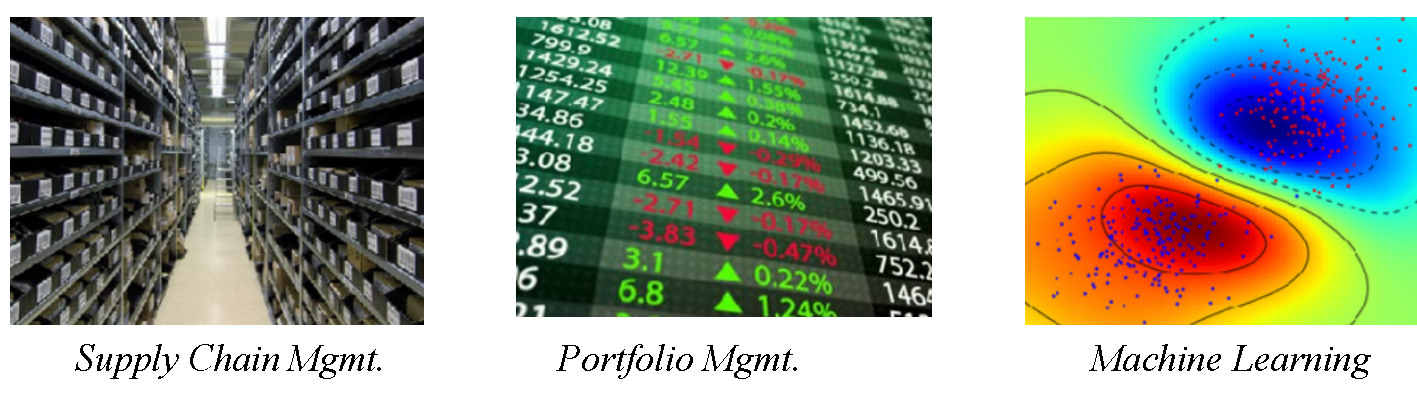
\includegraphics[width=0.23\textwidth]{figures/p_3}
\end{figure}
\item
{
\LARGE
Sample Average Approximation~(SAA):
\[
\begin{array}{ll}
\displaystyle
\inf_{\theta\in\Theta}&\quad \big\{
\mathcal{R}(\theta;\widehat{\mathbb{P}}_n) \triangleq \mathbb{E}_{\widehat{\mathbb{P}}_n}\big[f_{\theta}(z)\big]
\big\},\quad \text{where }\widehat{\mathbb{P}}_n=\frac{1}{n}\sum_{i=1}^n\delta_{\hat{x}_i}.
\end{array}
\] 
}
\item
{
\LARGE
Wasserstein Distributionally Robust Optimization~(DRO):
\[
\begin{array}{ll}
\inf\limits_{\theta\in\Theta}&\quad \left\{
\sup\limits_{\mathbb{P}\in\mathcal{P}}~\mathbb{E}_{\mathbb{P}}\big[f_{\theta}(z)\big]
\right\},~~ \text{where }
\mathcal{P} = \big\{
\mathbb{P}:~W(\widehat{\mathbb{P}}, \mathbb{P})\le \rho
\big\}.
\end{array}
\]
}
\item
{
\LARGE
Facts about Wasserstein DRO:\vspace{0.1in} 
\begin{itemize}
\item
For WDRO with $n$-point nominal distribution, the worst-case distribution is supported on $n+1$ points.\vspace{0.1in} 
\item
Finite-dimensional convex reformulation is available if the objective is a pointwise maximum of finitely many concave functions.\vspace{0.1in} 
\item
Some cases the same performance as SAA.
\end{itemize}
}
\end{itemize}
\vspace{0.5in} 
\newpage
\mysection{Sinkhorn Distance and Robust Formulation}
\vspace{0.1in}
\begin{itemize}
\item
{
\LARGE
Sinkhorn Distance~[Cuturi 2013]: 
\[
\mathcal{W}_{\color{red}\Reg}(\bP, \bQ) \:= \inf_{
\substack{
\gamma\in\Gamma(\bP, \bQ)
}}~ \left\{\mathbb{E}_{(X,Y)\sim\gamma}[c(X,Y)] + {\color{red}\Reg H(\gamma\mid\bP\otimes\nu)}\right\}.
\]}
\vspace{0.05in}
\item
{
\LARGE
Relative Entropy between $\gamma$ and $\bP\otimes\nu$:
\[
{\color{red}H(\gamma\mid\bP\otimes\nu) = \int \log\left(\frac{\diff\gamma(x,y)}{\diff\bP(x)\diff\nu(y)}\right)\diff\gamma(x,y).}
\]
}
\begin{figure}[H]
\centering
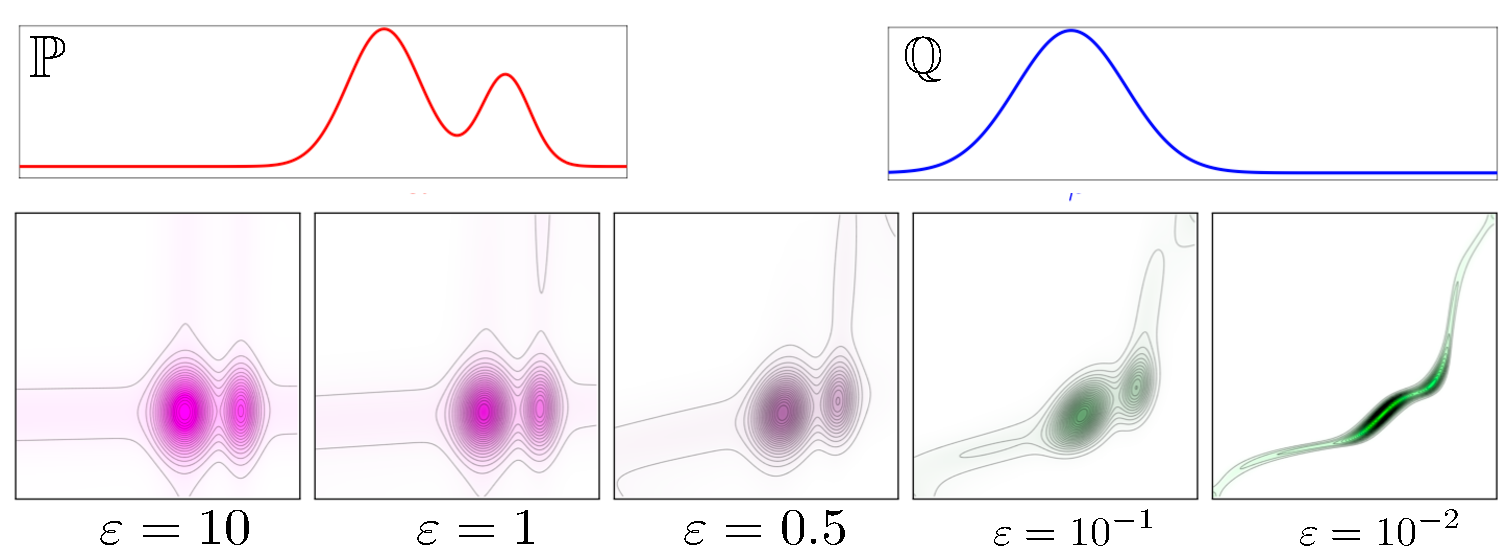
\includegraphics[width=0.23\textwidth]{figures/diagram_Sinkhorn}
\end{figure}
\vspace{0.1in}
\item
{
\LARGE
Sinkhorn DRO:
\[
\begin{aligned}
V^* = \inf_{\theta\in\Theta}&\sup_{\mathbb{P}\in\mathbb{B}_{\rho,\Reg}(\widehat{\mathbb{P}})}~
\mathbb{E}_{z\sim \mathbb{P}}[f_{\theta}(z)],\\
\text{where }&\mathbb{B}_{\rho,\Reg}(\widehat{\mathbb{P}})=\big\{
\mathbb{P}:~W_{\Reg}(\widehat{\mathbb{P}}, \mathbb{P})\le \rho
\big\}.
\end{aligned}
\]
}
\vspace{0.2in}
\item
\vspace{0.2in}
{
\LARGE
Visualization of Worst-Case Distributions:
}
\vspace{0.2in}
\begin{figure}[H]
\centering
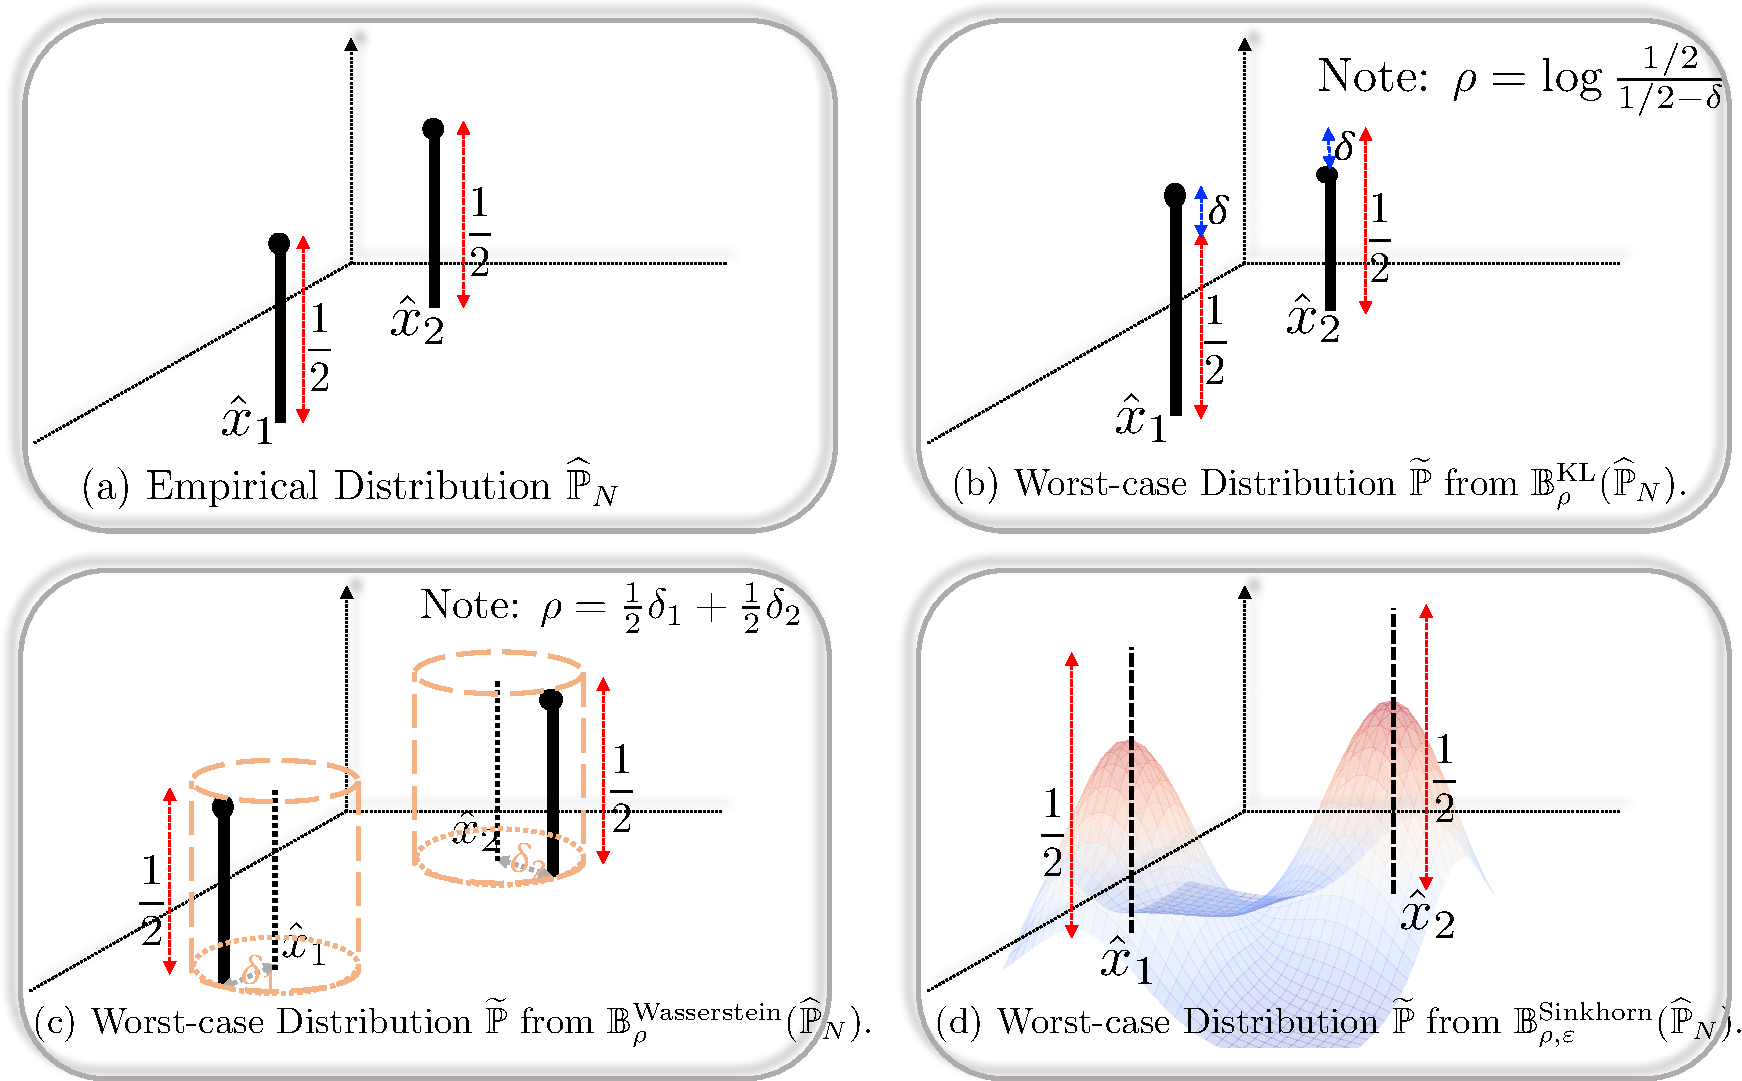
\includegraphics[width=0.23\textwidth]{figures/Fig_LFD}
\end{figure}
\end{itemize}











\newpage 
\begin{tcolorbox}[title=Theorem: Strong Dual Reformulation,
fonttitle=\LARGE\bfseries,
colback=red!5,colframe=red!65!black,
boxsep = 1mm, arc = 15pt, boxrule = 0.5pt,
boxrule=1pt,
toptitle=4mm,
  bottomtitle=4mm,
]
{
\LARGE
Assume that 
\begin{itemize}
    \item$\nu\{z:~0\le c(x,z)<\infty\}=1$ for $\widehat{\mathbb{P}}$-almost every $x$; 
    \item$\int e^{-c(x,z)/\Reg}\diff\nu(z) <\infty$ for $\widehat{\mathbb{P}}$-almost every $x$;
    \item$\mathcal{Z}$ is a measurable space, and the function $f:~\mathcal{Z}\to\mathbb{R}\cup\{\infty\}$ is measurable.
\end{itemize}
Then $V_{\text{P}} = V_{\text{D}}$:
\begin{equation*}
\begin{aligned}
V_{\text{P}}
&=\sup_{\mathbb{P}}~
\left\{\mathbb{E}_{z\sim \mathbb{P}}[f(z)]:\quad
W_{{\Reg}}(\widehat{\mathbb{P}}, \mathbb{P})\le \rho
\right\},\\
V_{\text{D}}
&=
\inf_{\lambda>0}~\lambda\overline{\rho}+\lambda{\Reg}\int_{\Omega}\log\left(
\mathbb{E}_{\bQ_x}\left[ 
e^{f(z)/(\lambda{\Reg})}
\right]\right)\diff\widehat{\mathbb{P}}(x),
\end{aligned}
\end{equation*}
where
\[
\begin{aligned}
 \overline{\rho} &= \rho+{\Reg}\int_{\Omega}\log\left(\int_{\Omega}e^{-c(x,z)/{\Reg}}\diff\nu(z)\right)\diff\widehat{\mathbb{P}}(x),
 \\
\diff\bQ_{x}(z) &= \frac{e^{-c(x,z)/{\Reg}}}{\int_{\Omega}e^{-c(x,u)/{\Reg}}\diff\nu(u)}\diff\nu(z).
\end{aligned}
\]
}
\end{tcolorbox}




















{
\LARGE
{\bf Proof Sketch of Strong Duality}
\begin{enumerate}
\item
First show the {\color{blue}weak duality} result $V_{\text{P}}\le V_{\text{D}}$.
\item
Construct {\color{blue}primal feasible solution $\widetilde{\bP}$} with $V_{\text{P}}\ge\mathbb{E}_{z\sim \widetilde{\bP}}[f(z)]=V_{\text{D}}$.
\end{enumerate}
{\color{purple}
{\bf Geometry of Worst-Case Distribution: }}
\begin{itemize}
\item
For each $x\in\text{supp}(\widehat{\mathbb{P}})$, optimal transport maps it to a (conditional) distribution $\gamma_x$:
\[
\frac{\diff\gamma_x(z)}{\diff\nu(z)}=
  \alpha_x\cdot\exp\Big(\big( 
  f(z) - \lambda^\ast c(x,z) \big)/(\lambda^\ast\Reg)\Big).
\]
\item
Worst-case distribution $\widetilde{\bP} = \int \gamma_x \diff\hP(x)$. 
\end{itemize}
}


\mysection{
 Algorithm for Sinkhorn Robust Learning
}

{
\LARGE
\vspace{-0.8in} 
\[
V^* = \min_{\lambda\ge0}~\left\{
\lambda\orho+ {\color{red}\underbrace{\min_{\theta\in\Theta}~\mathbb{E}_{x\sim \hP}~
\left[
\lambda\Reg\log\left(
\mathbb{E}_{z\sim \bQ_{x}}\left[ 
e^{f_{\theta}(z)/(\lambda\Reg)}
\right]\right)
\right]}_{V(\lambda)}}
\right\}
\]
{\bf Bisection Search on $\lambda$: }
Estimating $V(\lambda)$ up to accuracy $O(\delta)$ for $O(\text{Poly}(\log\frac{1}{\delta}))$ times to find $\delta$-optimal solution of $V^*$.
}
\newpage
{
\LARGE
{\bf Stochastic Approximation for Solving $V(\lambda)$}
\begin{itemize}
\item
Goal: to solve the optimization
\[
\min_{\theta\in\Theta}~\left\{F(\theta):=\mathbb{E}_{x\sim \hP}~
\left[
\lambda\Reg\log\left(
\mathbb{E}_{z\sim \bQ_{x}}\left[ 
e^{f_{\theta}(z)/(\lambda\Reg)}
\right]\right)
\right]\right\}.
\]
\item
Biased Stochastic Mirror Descent~(BSMD): for $t=1,\ldots,T$, 
\[
\left\{
\begin{aligned}
v(\theta_t)&\leftarrow \text{(biased) gradient/subgradient estimate of $F(\theta_t)$}\\
\theta_{t+1}&\leftarrow \textbf{Prox}_{\theta_t}\big(\gamma v(\theta_t)\big)
\end{aligned}
\right.
\]
{\bf Remark: Gradient estimators should {\color{blue}optimally} balance the {\color{blue}bias-variance} trade-off.}
\item
Complexity of finding $\delta$-optimal solution or $\delta$-critical point:
\begin{figure}[H]
\centering
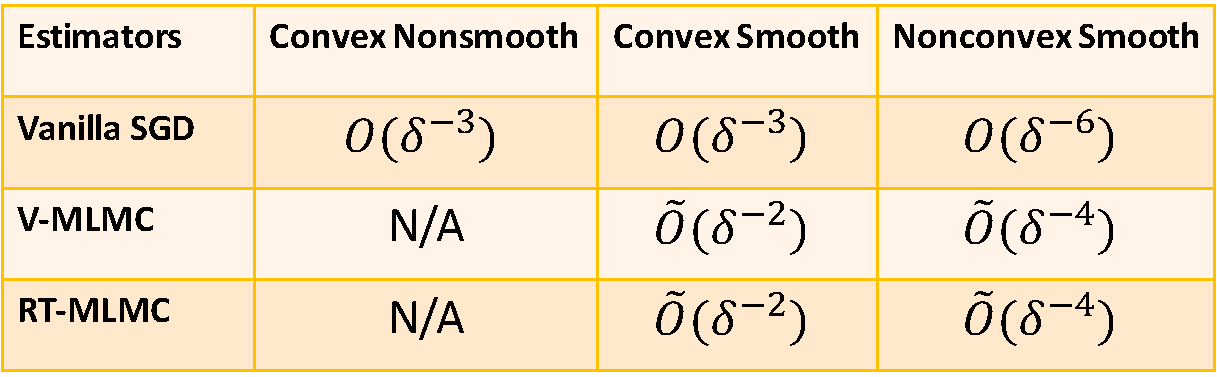
\includegraphics[width=0.21\textwidth]{figures/Fig_com}
\end{figure}
\end{itemize}
}









\mysection{Example: Mean-Risk  Portfolio Optimization}
\begin{figure}[H]
\centering
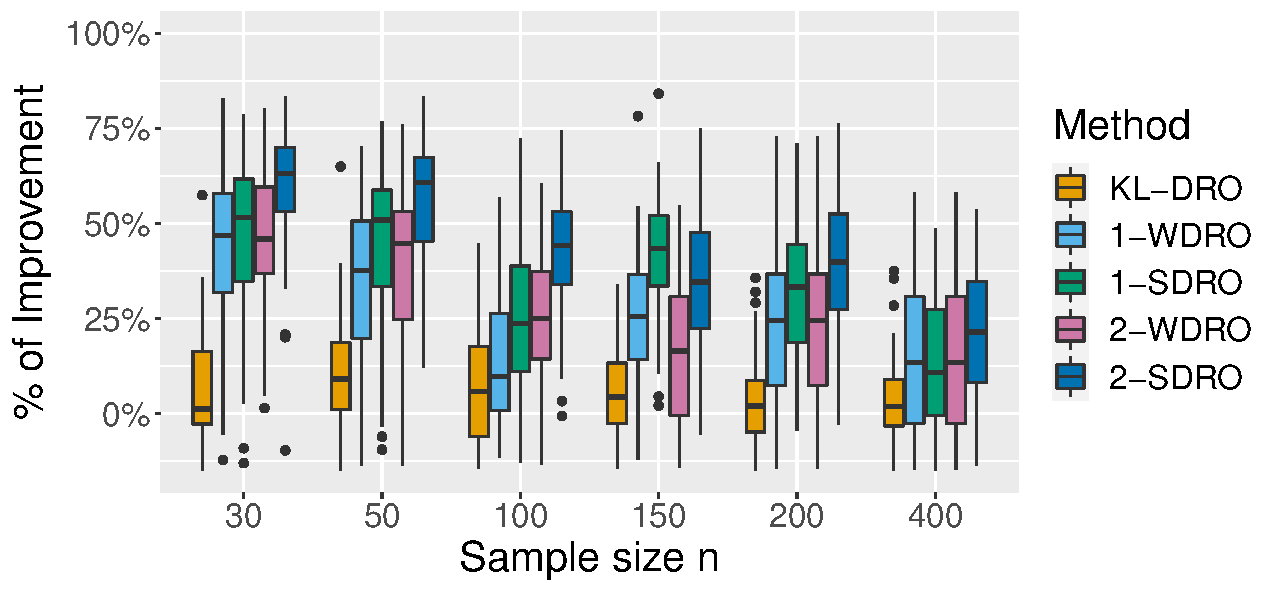
\includegraphics[width=0.22\textwidth]{figures/Risk_n}
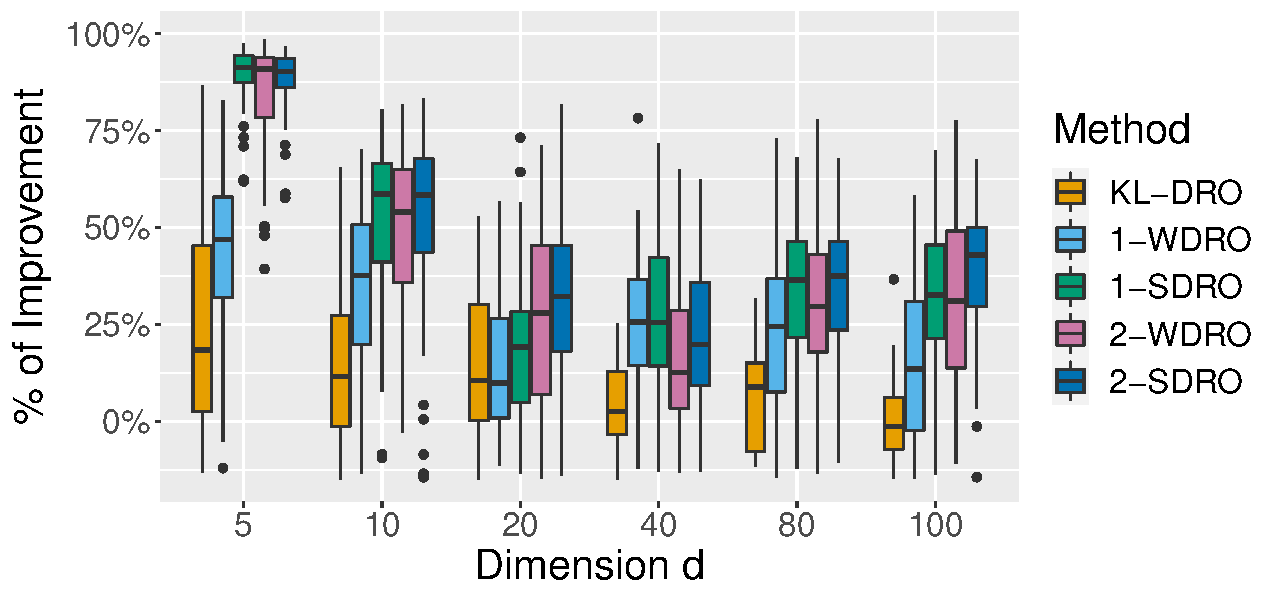
\includegraphics[width=0.22\textwidth]{figures/Risk_dim}
\end{figure}



\end{multicols}
\end{poster}

\end{document}

